Im folgenden Abschnitt sind die während des Versuchs aufgenommenen Messwerte,
sowie die daraus berechneten Ergebnisse tabellarisch und graphisch dargestellt.
Die erhaltenen Fehler der Ergebnisse wurden mit Hilfe der in \cref{sec:Fehlerrechnung}
aufgestellten Fehlergleichungen berechnet.


\subsection{Messung des Nulleffekts}

	Die Messung des Nulleffekt über einen Zeitraum von $T = \SI{900}{\second}$ 
	ergab die Anzahl der Zerfälle pro Intervall $\Delta t$ 
	\begin{empheq}{align}
		\notag
		N_{0} &= \dfrac{306}{900}\ \si{\per\second} \cdot \Delta t\\    
		&= \SI{0.34}{\per\second}  \cdot \Delta t. 
	\end{empheq} 

\subsection{Bestimmung der Halbwertszeiten der zwei möglichen Zerfälle von Rhodium}
	
	Die bei der Messung des Zerfalls von Rhodium aufgenommenen Messwerte
	für die Zeit $t$ und die Anzahl der gemessenen Zerfälle $N$ in \cref{tab:Auswertung_Messwerte_Rhodium}
	eingetragen. Auch die um den, vor dem Versuch bestimmte Nulleffekt $N_{0}$
    verringerte Anzahl an Zerfällen ist zusammen mit dem natürlichen Logarithmus
    aus diesen Werten in \cref{tab:Auswertung_Messwerte_Rhodium} zu finden.
    Die angegebenen Messfehler wurden mittels \cref{std:Abweichung Messwerte} berechnet.
    
   	\begin{table}[!h]
	\centering
	\begin{adjustbox}{width=1\textwidth, center}
	\begin{tabular}{|r|c|c|c|r|c|c|c|}
		\hline
		Zeit & Zerfälle & Zerfälle & ln der Zerfälle & Zeit & Zerfälle & Zerfälle & ln der Zerfälle\\
		$t$ [\si{\second}] & $N$ & $N - N_{0}$ & $\ln(N - N_{0})$ & $t$ [\si{\second}] & $N$ & $N - N_{0}$ & $\ln(N - N_{0})$\\
\hline\hline
		\num{20} & \num{1.9(1)e+02} & \num{1.9(1)e+02} & \num{5.24(7)} & \num{380} & \num{36(6)} & \num{29(5)} & \num{3.4(2)}\\
		\num{40} & \num{1.6(1)e+02} & \num{1.5(1)e+02} & \num{5.03(8)} & \num{400} & \num{48(7)} & \num{41(6)} & \num{3.7(2)}\\
		\num{60} & \num{1.5(1)e+02} & \num{1.4(1)e+02} & \num{4.97(8)} & \num{420} & \num{36(6)} & \num{29(5)} & \num{3.4(2)}\\
		\num{80} & \num{9(1)e+01} & \num{86(9)} & \num{4.5(1)} & \num{440} & \num{43(7)} & \num{36(6)} & \num{3.6(2)}\\
		\num{100} & \num{1.1(1)e+02} & \num{1.1(1)e+02} & \num{4.7(1)} & \num{460} & \num{30(5)} & \num{23(5)} & \num{3.1(2)}\\
		\num{120} & \num{84(9)} & \num{77(9)} & \num{4.3(1)} & \num{480} & \num{38(6)} & \num{31(6)} & \num{3.4(2)}\\
		\num{140} & \num{1.0(1)e+02} & \num{89(9)} & \num{4.5(1)} & \num{500} & \num{29(5)} & \num{22(5)} & \num{3.1(2)}\\
		\num{160} & \num{75(9)} & \num{68(8)} & \num{4.2(1)} & \num{520} & \num{27(5)} & \num{20(4)} & \num{3.0(2)}\\
		\num{180} & \num{61(8)} & \num{54(7)} & \num{4.0(1)} & \num{540} & \num{32(6)} & \num{25(5)} & \num{3.2(2)}\\
		\num{200} & \num{76(9)} & \num{69(8)} & \num{4.2(1)} & \num{560} & \num{22(5)} & \num{15(4)} & \num{2.7(3)}\\
		\num{220} & \num{48(7)} & \num{41(6)} & \num{3.7(2)} & \num{580} & \num{20(4)} & \num{13(4)} & \num{2.6(3)}\\
		\num{240} & \num{62(8)} & \num{55(7)} & \num{4.0(1)} & \num{600} & \num{35(6)} & \num{28(5)} & \num{3.3(2)}\\
		\num{260} & \num{46(7)} & \num{39(6)} & \num{3.7(2)} & \num{620} & \num{33(6)} & \num{26(5)} & \num{3.3(2)}\\
		\num{280} & \num{49(7)} & \num{42(6)} & \num{3.7(2)} & \num{640} & \num{21(5)} & \num{14(4)} & \num{2.7(3)}\\
		\num{300} & \num{52(7)} & \num{45(7)} & \num{3.8(1)} & \num{660} & \num{14(4)} & \num{7(3)} & \num{2.0(4)}\\
		\num{320} & \num{55(7)} & \num{48(7)} & \num{3.9(1)} & \num{680} & \num{19(4)} & \num{12(3)} & \num{2.5(3)}\\
		\num{340} & \num{51(7)} & \num{44(7)} & \num{3.8(2)} & \num{700} & \num{24(5)} & \num{17(4)} & \num{2.8(2)}\\
		\num{360} & \num{45(7)} & \num{38(6)} & \num{3.6(2)} & \num{720} & \num{22(5)} & \num{15(4)} & \num{2.7(3)}\\
		\hline
	\end{tabular}
    \end{adjustbox}
	\caption{Gemessene Anzahl der Zerfäll, Anzahl der Zerfälle nach Subtraktion des Nulleffekts und Werte des natürlichen Logarithmusses von diesen \label{tab:Auswertung_Messwerte_Rhodium}}
\end{table}
 
   	
   	In \cref{fig:} ist die logarithmierten Anzahl der Zerfälle $\Ln{N - N_{0}}$ aus \cref{tab:Auswertung_Messwerte_Rhodium} gegen die Zeit $t$ aufgetragen.  
   	
    \includeFigure[scale=0.7]{Grafiken/Messwerte_Rh.pdf}{Graphische Darstellung der logarithmierten Zerfälle ohne den Nulleffekt}{\label{fig:Auswertung_Messwerte_Rh}}
     
    Der Zeitpunkt ab dem nur noch der Zerfall mit der höheren Halbwertzeit messbar ist
    wurde für die folgenden Berechnungen $t^{*} = \SI{480}{\second}$ gewählt.
    Die Messwerte für $t > t*$ sind noch einmal in \cref{tab:Auswertung_Messwerte_Rhodium_lang} gelistet und 
    in  \cref{fig:Auswertung_Messwerte_Rh_lang} graphisch dargestellt. Diese Darstellung ist um die Regressiongerade
    dieser Messwerte ergänzt dir mittels \emph{SciPy} \cite{SciPy} berechnet wurde.
    Die lineare Regression für den Ansatz
    \begin{empheq}{equation}
    \Ln{N} = \lambda_{l} \cdot t + c_{l},
    \end{empheq}
    ergibt die Parameter
    \addtocounter{equation}{-1}
    \begin{subequations}
    	\begin{empheq}{align}
    		\lambda_{l} &= \SI{0.003(2)}{\per\second} \quad \text{und} \\
    		c_{l} &= \SI{4.4(9)}{}.
    	\end{empheq}
    \end{subequations}

	\begin{table}[!h]
	\centering
	\begin{tabular}{|r|c|c|}
		\hline
		Zeit & Zerfälle & ln der Zerfälle\\
		$t$ [\si{\second}] & $N_{l}$ & $\ln(N - N_{0})$\\
\hline\hline
		\num{420} & \num{29(5)} & \num{3.4(2)}\\
		\num{440} & \num{36(6)} & \num{3.6(2)}\\
		\num{460} & \num{23(5)} & \num{3.1(2)}\\
		\num{480} & \num{31(6)} & \num{3.4(2)}\\
		\num{500} & \num{22(5)} & \num{3.1(2)}\\
		\num{520} & \num{20(4)} & \num{3.0(2)}\\
		\num{540} & \num{25(5)} & \num{3.2(2)}\\
		\num{560} & \num{15(4)} & \num{2.7(3)}\\
		\num{580} & \num{13(4)} & \num{2.6(3)}\\
		\num{600} & \num{28(5)} & \num{3.3(2)}\\
		\num{620} & \num{26(5)} & \num{3.3(2)}\\
		\num{640} & \num{14(4)} & \num{2.7(3)}\\
		\num{660} & \num{7(3)} & \num{2.0(4)}\\
		\num{680} & \num{12(3)} & \num{2.5(3)}\\
		\num{700} & \num{17(4)} & \num{2.8(2)}\\
		\num{720} & \num{15(4)} & \num{2.7(3)}\\
		\hline
	\end{tabular}
	\caption{Messwerte zur Bestimmung der Halbwertszeit des langlebigen Zerfalls für t > t* \label{tab:Auswertung_Messwerte_Rhodium_lang}}
\end{table}


    \includeFigure[scale=0.7]{Grafiken/Messwerte_Rh_langlebig.pdf}{Graphische Darstellung der logarithmierten Zerfälle für $t > t^{*}$ }{\label{fig:Auswertung_Messwerte_Rh_lang}}
    
    Dabei gilt $c_{l} = \Ln{N_{a}(1 - \E{-\lambda_{l}\Delta t})}$ und somit erhält man hieraus
    die gesuchte Konstante, mit dem Fehler nach \cref{std:Exp},
   	\begin{empheq}{equation}
   		\E{c_{l}} = N_{a}(1 - \E{-\lambda_{l}\Delta t}) = \SI{70(70)}{}.
   	\end{empheq}
   	
   	Aus der erhaltenen Steigung $\lambda_{l}$ der Regressionsgerade, welche der 
   	Zerfallskonstante des langlebigeren Zerfalls entspricht, lässt sich mit 
   	Hilfe von \cref{eq:Theorie_Halbwertzeit} dessen Halbwertzeit zu
  	\begin{empheq}{equation}
  		t_{\sfrac{1}{2},l} =  \SI{277(168)}{\second}
  	\end{empheq}
    bestimmen. Der angegebene Fehler errechnet sich \cref{std:Halbwertszeit}.\\
    
    Durch die zuvor bestimmten Parameter ist es nun möglich, das Zerfallsgesetz für die langlebigeren Kerne
    aufzustellen und somit die Zerfallskurve vor dem Zeitpunkt $t*$ zu bestimmen. Durch Subtraktion dieser
    Zerfälle von den Messwerten für $t << t*$ erhält man die Zerfälle der kurzlebigen Kerne. Die Ergebnisse
    dieses Vorgehens sind in \cref{tab:Auswertung_Messwerte_Rhodium_kurz} zu finden und in \cref{fig:Auswertung_Messwerte_Rh_kurz} graphisch dargestellt.
    
    \begin{table}[!h]
	\centering
	\begin{tabular}{|r|c|c|c|}
		\hline
		Zeit & Zerf�lle & Zerf�lle & ln der Zerf�lle\\
		$t$ [\si{\second}] & $N$ & $N - N_{l}$ & $\ln(N - N_{0})$\\
\hline\hline
		\num{20} & \num{1.9(1)e+02} & \num{1.1(2)e+02} & \num{4.7(1)}\\
		\num{40} & \num{1.5(1)e+02} & \num{8(1)e+01} & \num{4.4(2)}\\
		\num{60} & \num{1.4(1)e+02} & \num{8(1)e+01} & \num{4.3(2)}\\
		\num{80} & \num{86(9)} & \num{2(1)e+01} & \num{3.1(5)}\\
		\num{100} & \num{1.1(1)e+02} & \num{5(1)e+01} & \num{3.8(3)}\\
		\num{120} & \num{77(9)} & \num{2(1)e+01} & \num{3.0(6)}\\
		\num{140} & \num{89(9)} & \num{3(1)e+01} & \num{3.5(3)}\\
		\num{160} & \num{68(8)} & \num{2(1)e+01} & \num{2.8(7)}\\
		\num{180} & \num{54(7)} & \num{0(1)e+01} & \num{2(2)}\\
		\num{200} & \num{69(8)} & \num{2(1)e+01} & \num{3.1(5)}\\
		\hline
	\end{tabular}
	\caption{Messwerte zur Bestimmung der Halbwertszeit des langlebigen Zerfalls f�r t << t* \label{tab:Auswertung_Messwerte_Rhodium_kurz}}
\end{table}

    
    \includeFigure[scale=0.7]{Grafiken/Messwerte_Rh_kurzlebig.pdf}{Graphische Darstellung der logarithmierten Zerfälle% 
    für $t << t^{*}$ }{\label{fig:Auswertung_Messwerte_Rh_kurz}} 
     
    Aus der, mit \emph{SciPy} durchgeführten, linearen Regression mit dem Ansatz
    \begin{empheq}{equation}
    \Ln{N} = \lambda_{k} \cdot t + c_{k},
    \end{empheq}
    ergeben sich die Parameter zu
    \addtocounter{equation}{-1}
    \begin{subequations}
       	\begin{empheq}{align}
       		\lambda_{k} &= \SI{0.013(3)}{\per\second} \quad \text{und} \\
       		c_{k} &= \SI{4.9(4)}{}.
       	\end{empheq}
    \end{subequations}  
    Die daraus erhaltene Gerade ist ebenfalls in \cref{fig:Auswertung_Messwerte_Rh_kurz} eingezeichnet.
    
    Analog zu dem Zerfall der langlebigeren Kerne, erhält man aus den bestimmten Regressionsparametern
    die gesuchte Konstante $\E{c_{k}}$ und die Halbwertzeit $t_{\sfrac{1}{2},k}$ dieses Zerfalls zu
    \begin{empheq}{align}
   		\E{c_{k}} &= N_{a}(1 - \E{-\lambda_{k}\Delta t}) = \SI{128(50)}{} \quad \text{und}\\
   		t_{\sfrac{1}{2},k} &=  \SI{54(13)}{\second}.
   	\end{empheq}
    Die angegebenen Fehler ergeben sich jeweils aus \cref{std:Exp} bzw. \cref{std:Halbwertszeit}. 
    
    
    Die auf diese Weise bestimmten Zerfallsgesetze sind in \cref{fig:Auswertung_Rh_Ergebniss} zusammen mit der Summe beider Zerfäll
    und den ursprünglichen Messwerten ohne den Nulleffekt aufgetragen.
    
    \includeFigure[scale=0.7]{Grafiken/Theoriekurven.pdf}{Graphische Darstellung der in der Auswertung bestimmten Zerfallsgesetze und deren summierter Zerfall im Vergleich zu den Messwerten}{\label{fig:Auswertung_Rh_Ergebniss}} 
     
\subsection{Bestimmung der Halbwertszeit von Indium}
Ziel dieses Abschnitts ist es, die Halbwertszeit von $^{116}$In zu ermitteln. Die notwendigen Messdaten und Ergebnisse sind im Folgenden sowohl tabellarisch als auch grafisch dargestellt. Bei diesem Teil des Experiments wurden die Zerfälle N nach Zeitintervallen von $\Delta t$=200s über einen Zeitraum von 60min notiert. 
Die Fehler der aufgenommenen und korrigierten Messwerte errechnen sich nach \cref{std:Abweichung Messwerte}.
%Bei der Korrektur um den Nulleffekt ergibt sich der Wert des resultierenden Fehlers erneut nach der Fehlerfortpflanzung zu $\sigma=\sqrt{\sigma_N^2+\sigma_{N_0}^2}$.

\begin{table}[htbp]
\centering\begin{tabular}{c|c|c|c|c|c|c}
$t [s]$ & $Zerfälle N$ & $\sigma_N$ & $N-N_0$ & $\sigma_{N-N_0}$ & $ln(N-N_0)$ & $\sigma_{ln}$\\
\hline \hline
200&	2853&	53&	2785&	54&	7.932&	0.019\\
400&  2617&	51&	2549&	52&	7.843&	0.020\\
600&	2535&	50&	2467&	51&	7.811&	0.021\\
800&	2355&	49&	2287&	49&	7.735&	0.022\\
1000&	2437&	49&	2369&	50&	7.770&	0.021\\
1200&	2233&	47&	2165&	48&	7.680&  0.022\\
1400&	2161&	46&	2093&	47&	7.646&	0.023\\
1600&	2149&	46&	2081&	47&	7.641&	0.023\\
1800&	1917&	44&	1849&	45&	7.522&	0.024\\
2000&	1816&	43&	1748&	43&	7.466&	0.025\\
2200&	1843&	43&	1775&	44&	7.482&	0.025\\
2400&	1639&	40&	1571&	41&	7.359&	0.026\\
2600&	1711&	41&	1643&	42&	7.404&	0.026\\
2800&	1625&	40&	1557&	41&	7.351&	0.026\\
3000&	1585&	40&	1517&	41&	7.324&	0.027\\
3200&	1432&	38&	1364&	39&	7.218&	0.028\\
3400&	1443&	38&	1375&	39&	7.226&	0.028\\
3600&	1358&	37&	1290&	38&	7.162&	0.029\\

\end{tabular}
\caption{Messdaten und Ergebnisse für die Bestimmung der Halbwertszeit von Indium}
\label{fig:Tab1}
\end{table}

\begin{figure}[htbp]
\centering{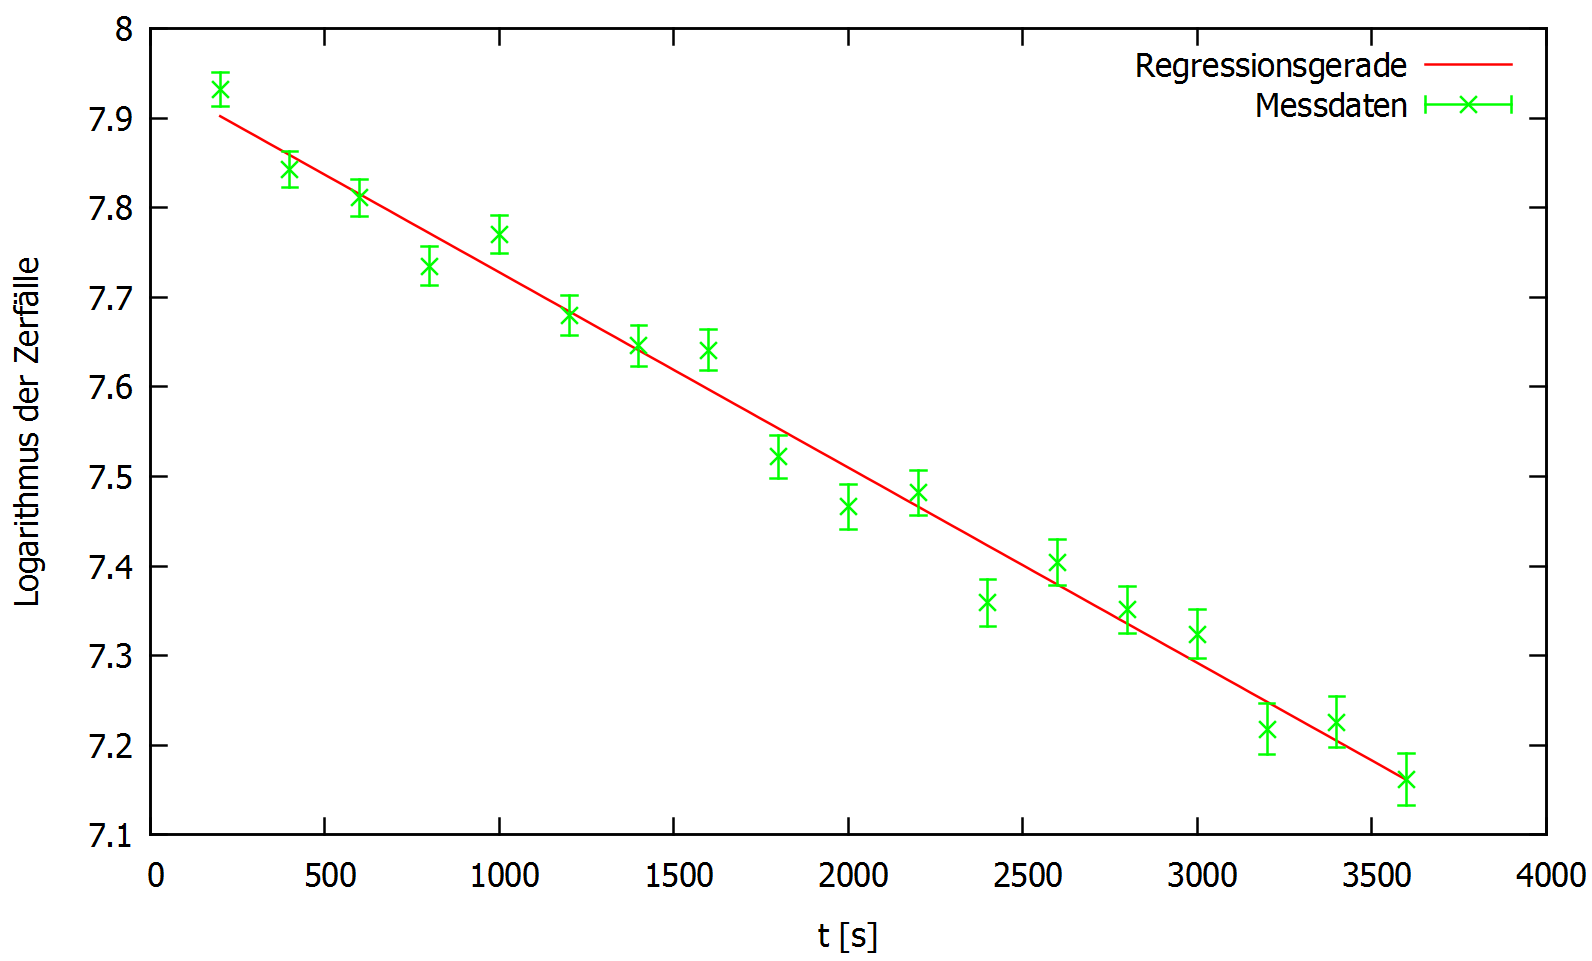
\includegraphics[scale=0.3]{Grafiken/702_Indium.PNG}}
\caption{Messdaten der Indium-Zerfälle mit Ausgleichsgerader}
\label{fig:Abbildung}
\end{figure}
Um nun die Zerfallskonstante $\lambda$ zu bestimmen wird eine lineare Ausgleichsrechnung durchgeführt. Hierbei werden die logarthmisierten Zerfälle als Funktion der Zeit aufgetragen und mithilfe von Gnuplot die Parameter einer Regressionsgeraden mit der Form f(x)=a$\cdot$x+b errechnet. Diese Form leitet sich aus der folgenden Gleichung her:
\begin{align*}
\ln(N-N_0)=\ln N_a(1-e^{-\lambda\Delta t})-\lambda t
\end{align*}
Hier ist $N_a$ die unbekannte Anzahl an Kernen der Indium Probe und $\Delta$t das Zeitintervall während der Messung. Die Parameter der Regressionsgeraden lauten:
\begin{align*}
\lambda&=0.000218\pm 0.000007s^{-1}\\
\ln N_0(1-e^{-\lambda\Delta t})&=7.946\pm0.0159\\
\end{align*}

Daraus lässt sich nun gemäß der Relation \cref{eq:Theorie_Halbwertzeit} die Halbzeit von Indium berechnen. Der Fehler ergibt sich durch Anwendung von \cref{std:Halbwertszeit}:

\begin{align*}
\rightarrow T_{1/2}=(3179.6\pm 102.1)s
\end{align*}